% !TeX program = xelatex
% !TeX encoding = UTF-8
% !TeX spellcheck = en_US
% !BIB program = biber
%% 
%%%%%%%%%%%%%%%%%%%%%%%%%%%%%%%%%%%%%%%%%%%%%%%%%%%%%%%%%%%%%%%%%%%%%%%%%%%%%%%%

%%%%%%%%%%%%%%%%%%%%%%%%%%%%%%%%%%%%%%%%%%%%%%%%%%%%%%%%%%%%%%%%%%%%%%%%%%%%%%%%
%% 
%%            JJJJ   K                         K   UUUU         UUUU  
%%            JJJJ   KKKK                   KKKK   UUUU         UUUU  
%%            JJJJ   KKKKKK               KKKKKK   UUUU         UUUU  
%%            JJJJ      KKKKKK         KKKKKK      UUUU         UUUU  
%%            JJJJ         KKKKKK   KKKKKK         UUUU         UUUU  
%%            JJJJ            KKKKKKKKK            UUUU         UUUU  
%%    JJ     JJJJJ               KKK               UUUUU       UUUUU  
%%  JJJJJJJJJJJJJ    KKKKKKKKKKKKKKKKKKKKKKKKKKK    UUUUUUUUUUUUUUU   
%%    JJJJJJJJJ      KKKKKKKKKKKKKKKKKKKKKKKKKKK      UUUUUUUUUUU     
%% 
%% This is an example file for using the JKU LaTeX technical report template
%% for your technical report.
%% 
%% Template created by Michael Roland (2021)
%% 
%%%%%%%%%%%%%%%%%%%%%%%%%%%%%%%%%%%%%%%%%%%%%%%%%%%%%%%%%%%%%%%%%%%%%%%%%%%%%%%%

%%%%%%%%%%%%%%%%%%%%%%%%%%%%%%%%%%%%%%%%%%%%%%%%%%%%%%%%%%%%%%%%%%%%%%%%%%%%%%%%
\documentclass[a4paper,oneside,10pt,ngerman]{scrartcl}
\usepackage[utf8]{inputenc}
\usepackage[
    TNF,
    equalmargins,
    techreport,
    nofancyfonts,
    logopath=../logos,
    fontpath=../fonts
]{../jkureport}
%% 
%%%%%%%%%%%%%%%%%%%%%%%%%%%%%%%%%%%%%%%%%%%%%%%%%%%%%%%%%%%%%%%%%%%%%%%%%%%%%%%%

%%%%%%%%%%%%%%%%%%%%%%%%%%%%%%%%%%%%%%%%%%%%%%%%%%%%%%%%%%%%%%%%%%%%%%%%%%%%%%%%
%% 
%% This is the place where you can load additional packages. If you want to load
%% a package `biblatex', you would use the command `\usepackage{biblatex}'.
%% 
\usepackage{enumerate}
\usepackage{listingsutf8}
\usepackage{graphicx}
\usepackage{siunitx}

%% 
%%%%%%%%%%%%%%%%%%%%%%%%%%%%%%%%%%%%%%%%%%%%%%%%%%%%%%%%%%%%%%%%%%%%%%%%%%%%%%%%

\newcommand{\designs}{../../designs}
\graphicspath{{images/}}

\begin{document}
%%%%%%%%%%%%%%%%%%%%%%%%%%%%%%%%%%%%%%%%%%%%%%%%%%%%%%%%%%%%%%%%%%%%%%%%%%%%%%%%
%% 
%% Report information and title page
%% 

\title{Inverter Verstärker}

\subtitle{UE - Technische Elektronik \\%
    \usekomafont{subtitlesmall}%
    \hfill\\%
    SoSe24\\
    \hfill\\%
}

\author{%
    Simon Grundner
    \affiliation{Institute for Integrated Circuits}
    \authornewline
    \authormail{k12136610@students.jku.at}
    \authorweb{https://jku.at/iic}
    \authornewline
}

\partnerlogo{../logos/iic}
\reportnumber{Aufgabe 1}
\setbottommark{Simon Grundner, k12136610}
\keywords{MOSFETs, Inverter-Verstärker, OSIC-Tools}

\maketitle
%% 
%%%%%%%%%%%%%%%%%%%%%%%%%%%%%%%%%%%%%%%%%%%%%%%%%%%%%%%%%%%%%%%%%%%%%%%%%%%%%%%%

\tableofcontents

%%%%%%%%%%%%%%%%%%%%%%%%%%%%%%%%%%%%%%%%%%%%%%%%%%%%%%%%%%%%%%%%%%%%%%%%%%%%%%%%
%% 
%% Add your report sections ...
%% 

\section{Inverter Verstärker}

\begin{highlightblock}[Aufgabe: Analyse eines Inverter-Verstärkers (PMOS/R)]
    Analysieren einen Inverter-Verstärker, der aus einem PMOS-Transistor und
    einem Widerstand besteht, unter Verwendung der sky130A-Technologie.
\end{highlightblock}

\subsection{Schaltung}

Links ist die PMOS-Transistor / Widerstand Verstärkerschaltung zu sehen. Als Last wird ein Widerstand von $R_L = \SI{50}{\kilo\ohm}$. Auf der Rechten Seite befindet sich das Modell des PMOS Transistors, welches für die Messung im Arbeitspunkt verwendet wird.

\begin{figure}[h]
    \centering
    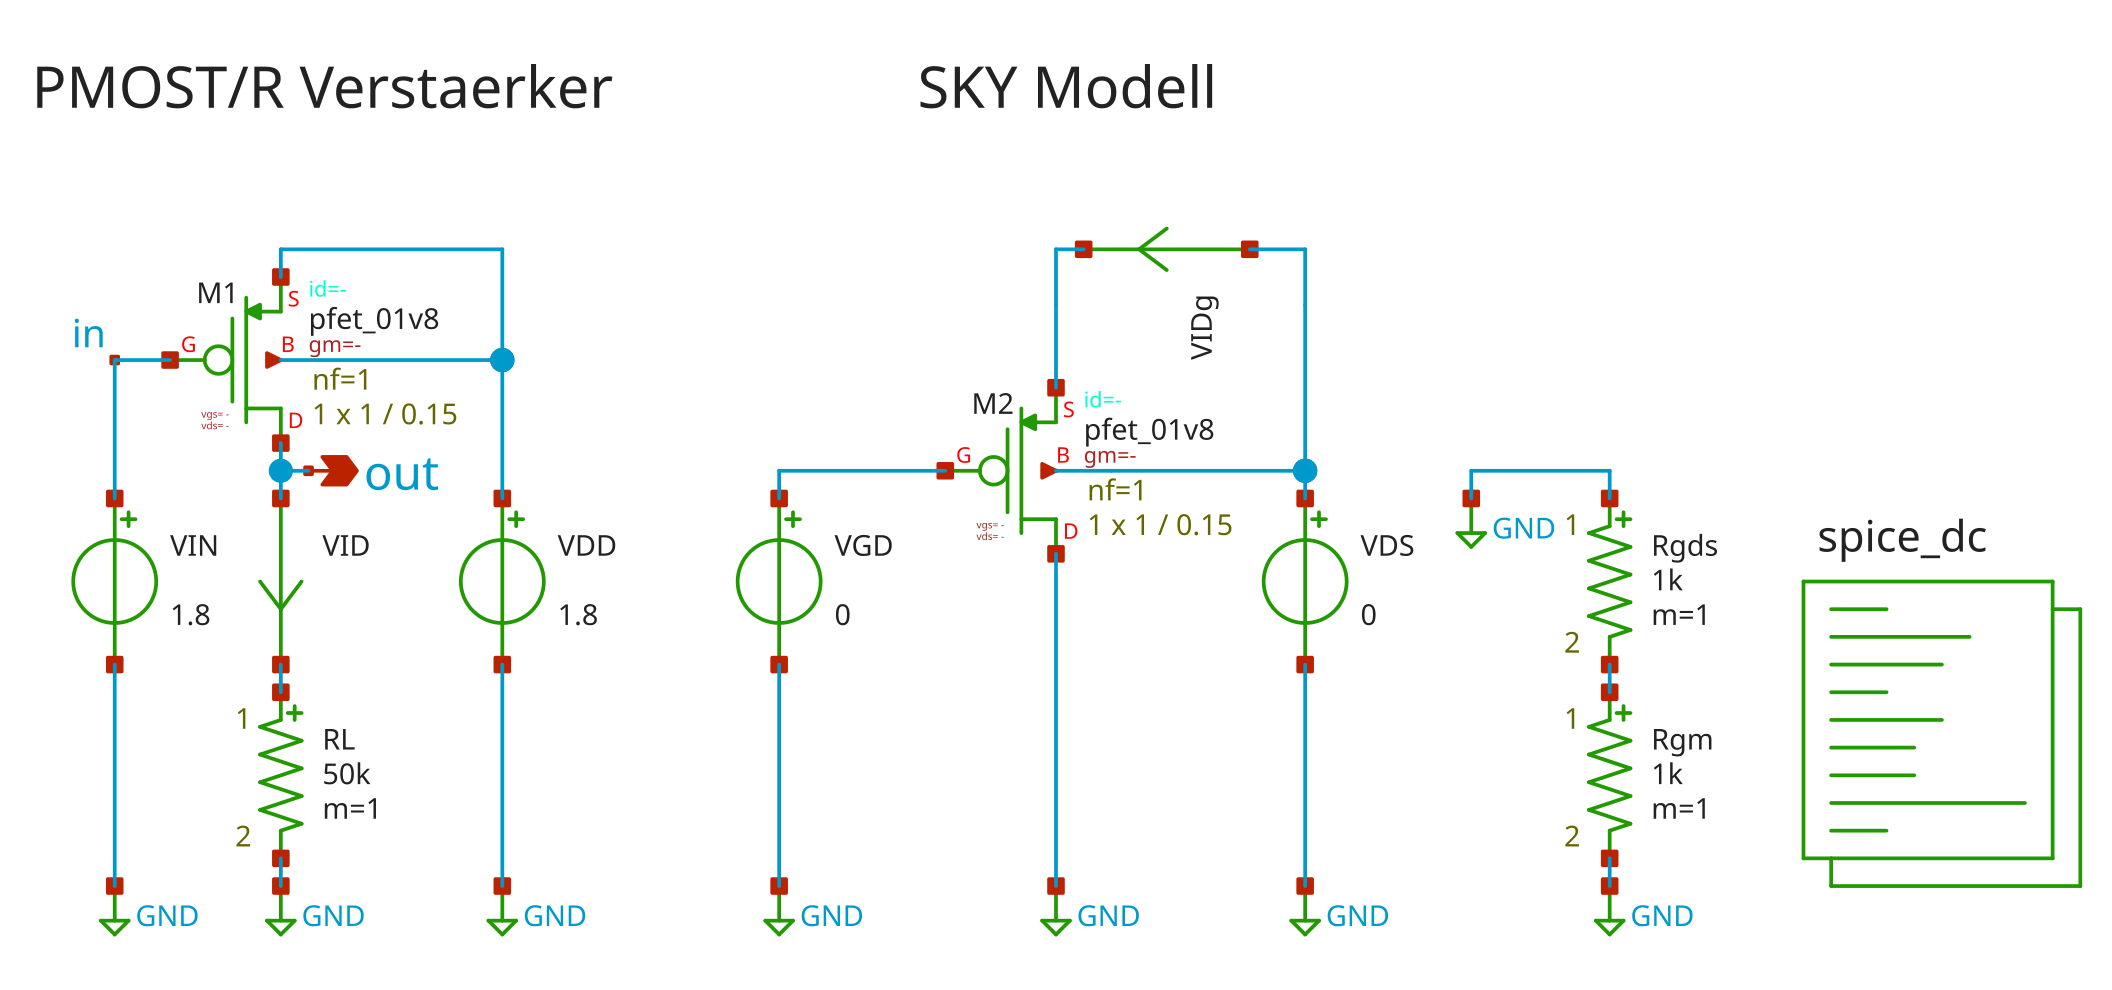
\includegraphics[width=0.8\textwidth]{plot-0.png}
    \caption{xschem Schaltung}\label{fig:xschem}
\end{figure}

\newpage
\subsection{Verstärkung und Arbeitspunkt}

Bei der PMOST/R Verstärkerschaltung wird der Arbeitspunktes bei maximaler Spannungsverstärkung
\[ A_0 = \frac{U_\mathrm{out}}{U_\mathrm{in}} \]
mittels DC sweep von \lstinline|VIN| ermittelt.

\lstinputlisting[firstline=77, lastline=81]{\designs/a1_k12136610.sch}

Nun werden die Spannungen bei der Maximalverstärkung gesucht und die Spannungsquellen im SKY Modell (\autoref{fig:xschem}) auf diesen Arbeitspunkt eingestellt.

\lstinputlisting[firstline=82, lastline=83]{\designs/a1_k12136610.sch}

\subsubsection{Ergebnisse}

In \autoref{fig:Uout-vs-Uin} ist das Inverter Verhalten der Schaltung zu erkennen und in \autoref{fig:A0-vs-Uin} der Verlauf der Spannungsverstärkung.

\begin{figure}[h]
    \begin{minipage}[t]{0.49\textwidth}
        \centering
        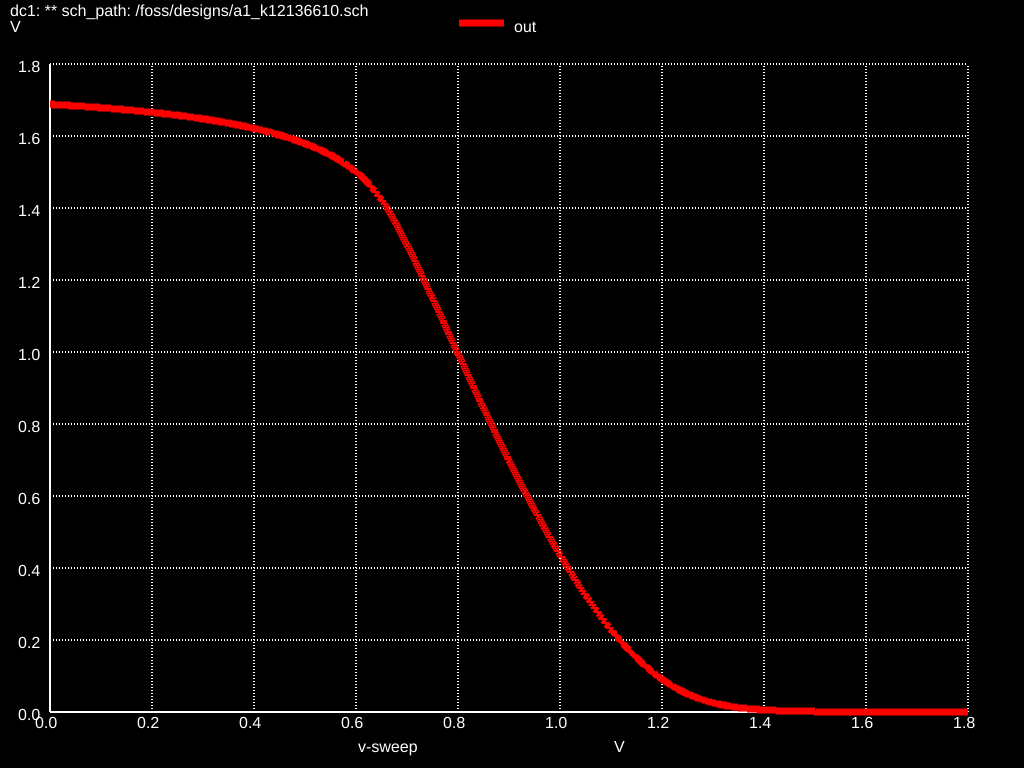
\includegraphics[width=\textwidth]{plot-2.png}
        \caption{Ausgangsspannung $U_\mathrm{out}$ vs $U_\mathrm{in}$}\label{fig:Uout-vs-Uin}
    \end{minipage}\hfill
    \begin{minipage}[t]{0.49\textwidth}
        \centering
        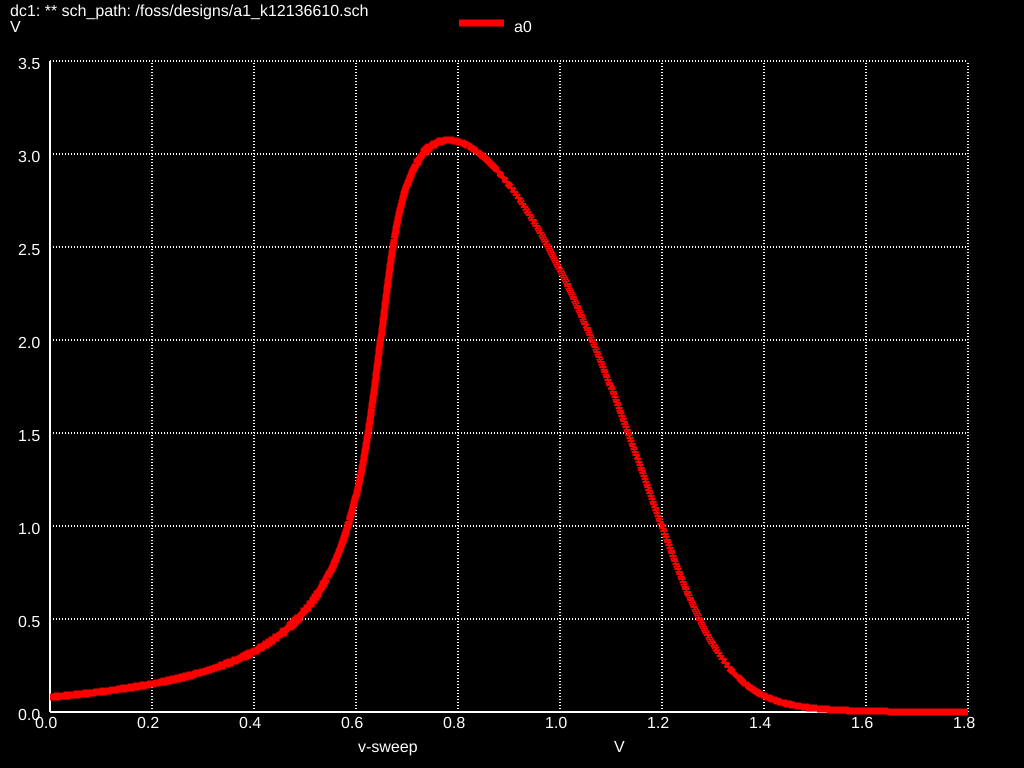
\includegraphics[width=\textwidth]{plot-1.png}
        \caption{Spannungsverstärkung $A_0$ vs $U_\mathrm{in}$}\label{fig:A0-vs-Uin}
    \end{minipage}
\end{figure}

Die Werte im Arbeitspunkt sind:

\begin{itemize}
    \item $A_{0, \max} = 3.07$
    \item $U_\mathrm{GD, op} = \SI{0.782}{\volt}$ (Eingangsspannung)
    \item $U_\mathrm{DS, op} = \SI{1.05}{\volt}$ (Biasspannung)
\end{itemize}

%% 
%%%%%%%%%%%%%%%%%%%%%%%%%%%%%%%%%%%%%%%%%%%%%%%%%%%%%%%%%%%%%%%%%%%%%%%%%%%%%%%%

\end{document}
\endinput
